\label{appendix:cuts}
This section contains reprensentation of the cuts necessary for the entire machine. See figure \ref{fig:cut01}, \ref{fig:cut02} and \ref{fig:cut03} for these representations. Please see the submitted .PDF files for the actual cutting files appropriate for a laser cutter. 
\begin{figure*}
	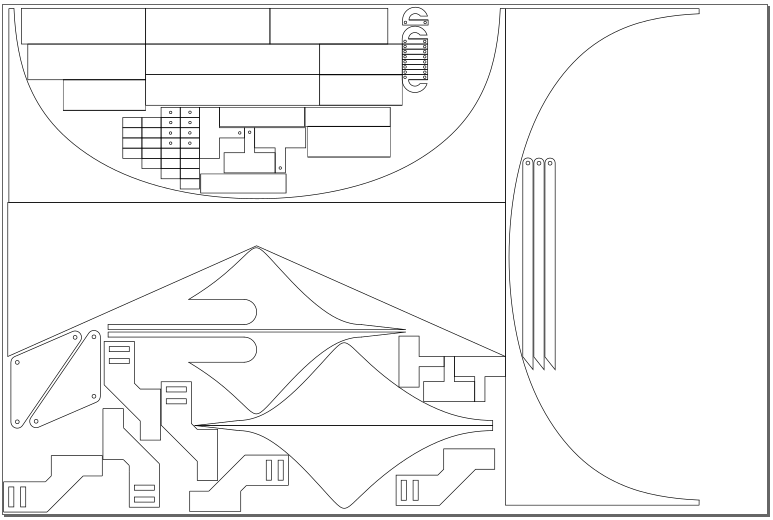
\includegraphics[width=\textwidth]{Cut01}
	\caption{This cut contains brackets and bodywork for the entire machine.}
	\label{fig:cut01}
\end{figure*}
\begin{figure*}
	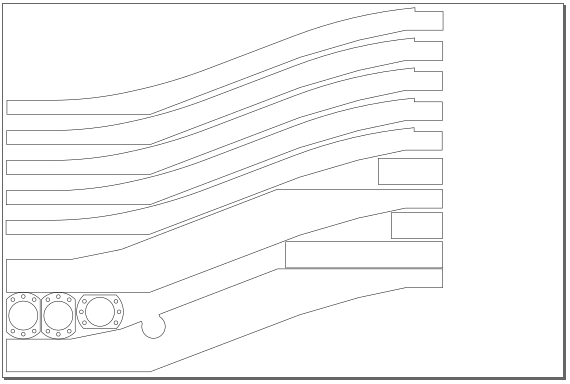
\includegraphics[width=\textwidth]{Cut02}
	\caption{This cut contains the cuts neccessary for the ball-return slide}
	\label{fig:cut02}
\end{figure*}
\begin{figure*}
	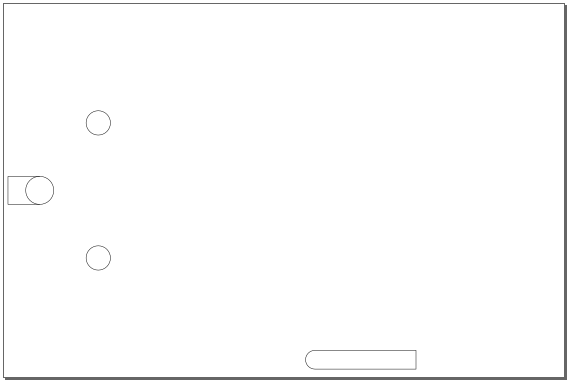
\includegraphics[width=\textwidth]{Cut03}
	\caption{This cut represents the holes neccesary for the playfield. Essentially when cut, the whole board becomes the playfield.}
	\label{fig:cut03}
\end{figure*}
